\section{Resultados}

En el artículo de Yuan Lin\cite{yuan_2009} se mencionan una serie de PDE con su solución análitica. Realizando una comparación de los resultados obtendios con el programa propio y los resultados de Yuan Lin, se obtuvo lo siguiente:

\subsection{Dataset 1}

Se tiene la siguiente ecuación diferencial parcial:

\begin{equation}
	\frac{\partial u}{\partial t} = \frac{\partial^2 u}{\partial x^2} \qquad 0<x<1, \; t>0 \label{eq:heat_1}
\end{equation}

con las siguientes condiciones de frontera:
\begin{equation}
	\begin{cases}
		u(x,0) & = sin(\pi x) \qquad 0<x<1 \\
		u(0,t) & =u(1,t) = 0, \qquad t>0
	\end{cases} \label{eq:bound_1}
\end{equation}

La solución análitica de este conjuntos de ecuaciones es:

\begin{equation}
	u(x,t)= e^{-\pi^2 t}sin(\pi x) \label{eq:sol_1}
\end{equation}

En la figura \ref{fig:sol_1} se muestra la solución análitica y numérica de la ecuación \ref{eq:bound_1} bajo las conficiones de frontera de la ecuación \ref{eq:bound_1}. La diferencia relativa entre los dos resultados es de 0.3531\%, dando así una gran similitud entre los dos resultados.

\begin{figure}[H]
	\centering
	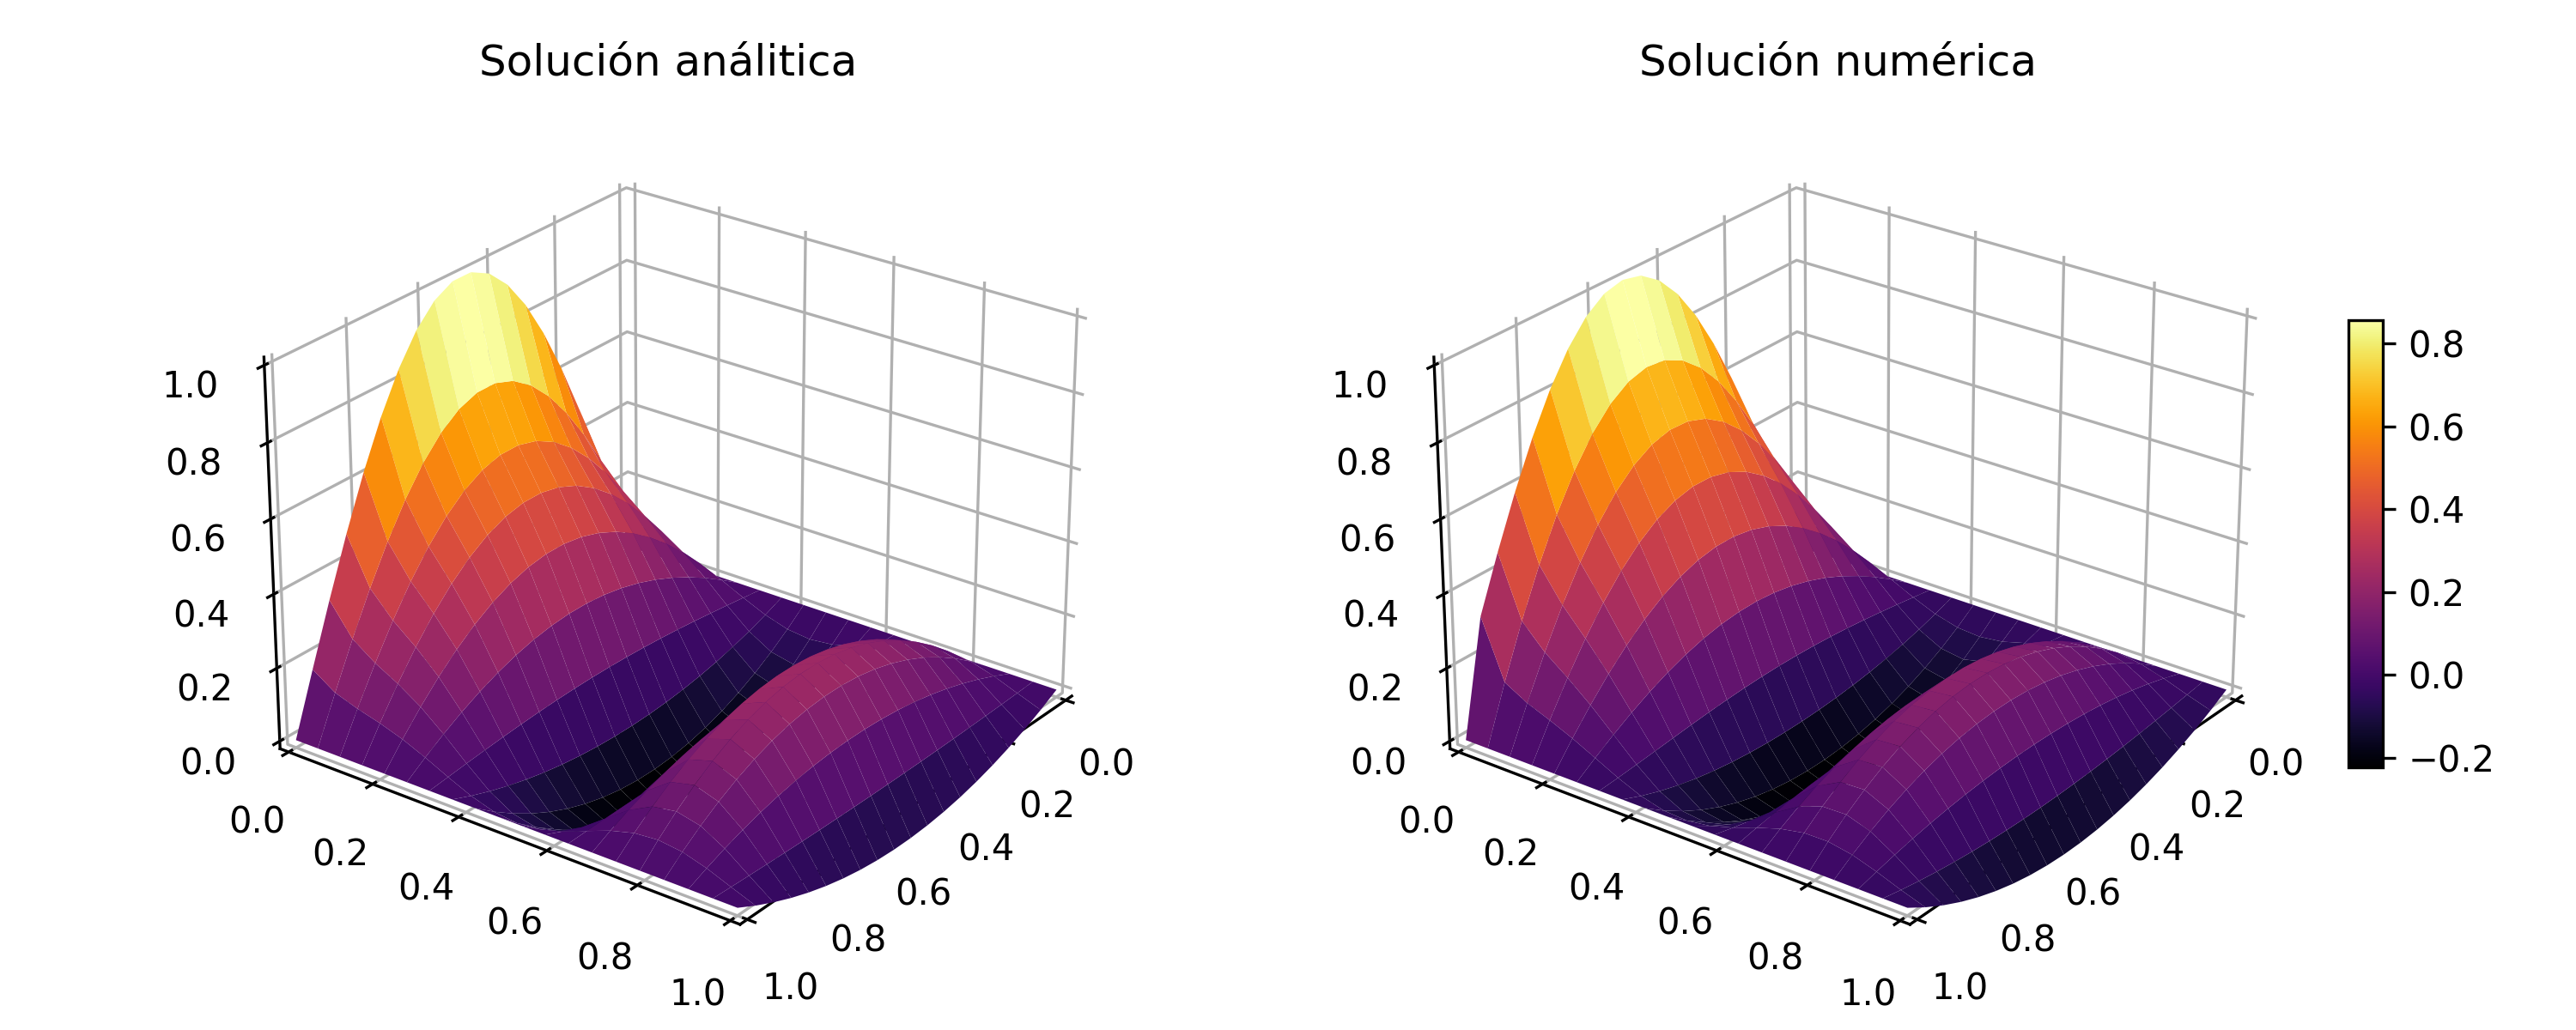
\includegraphics[width=17cm]{Graphics/surface_1.png}
	\caption{Solución análitica y numérica de la ecuación \ref{eq:heat_1} bajo las condiciones de frontera de la ecuación \ref{eq:bound_1}.}
	\label{fig:sol_1}
\end{figure}

\subsection{Dataset 2}

Se tiene la siguiente ecuación diferencial parcial:

\begin{equation}
	\frac{\partial u}{\partial t} = \frac{1}{\pi^2}\frac{\partial^2 u}{\partial x^2} \qquad 0<x<1, \; t>0 \label{eq:heat_2}
\end{equation}

con las siguientes condiciones de frontera:
\begin{equation}
	\begin{cases}
		u(x,0) & = sin(\pi x) \qquad 0<x<1 \\
		u(0,t) & =u(1,t) = 0, \qquad t>0
	\end{cases} \label{eq:bound_2}
\end{equation}

La solución análitica de este conjuntos de ecuaciones es:

\begin{equation}
	u(x,t)= e^{-t}sin(\pi x) \label{eq:sol_2}
\end{equation}

En la figura \ref{fig:sol_2} se muestra la solución análitica y numérica de la ecuación \ref{eq:bound_2} bajo las conficiones de frontera de la ecuación \ref{eq:bound_2}. La diferencia relativa entre los dos resultados es de 0.3512\%, dando así una gran similitud entre los dos resultados.

\begin{figure}[H]
	\centering
	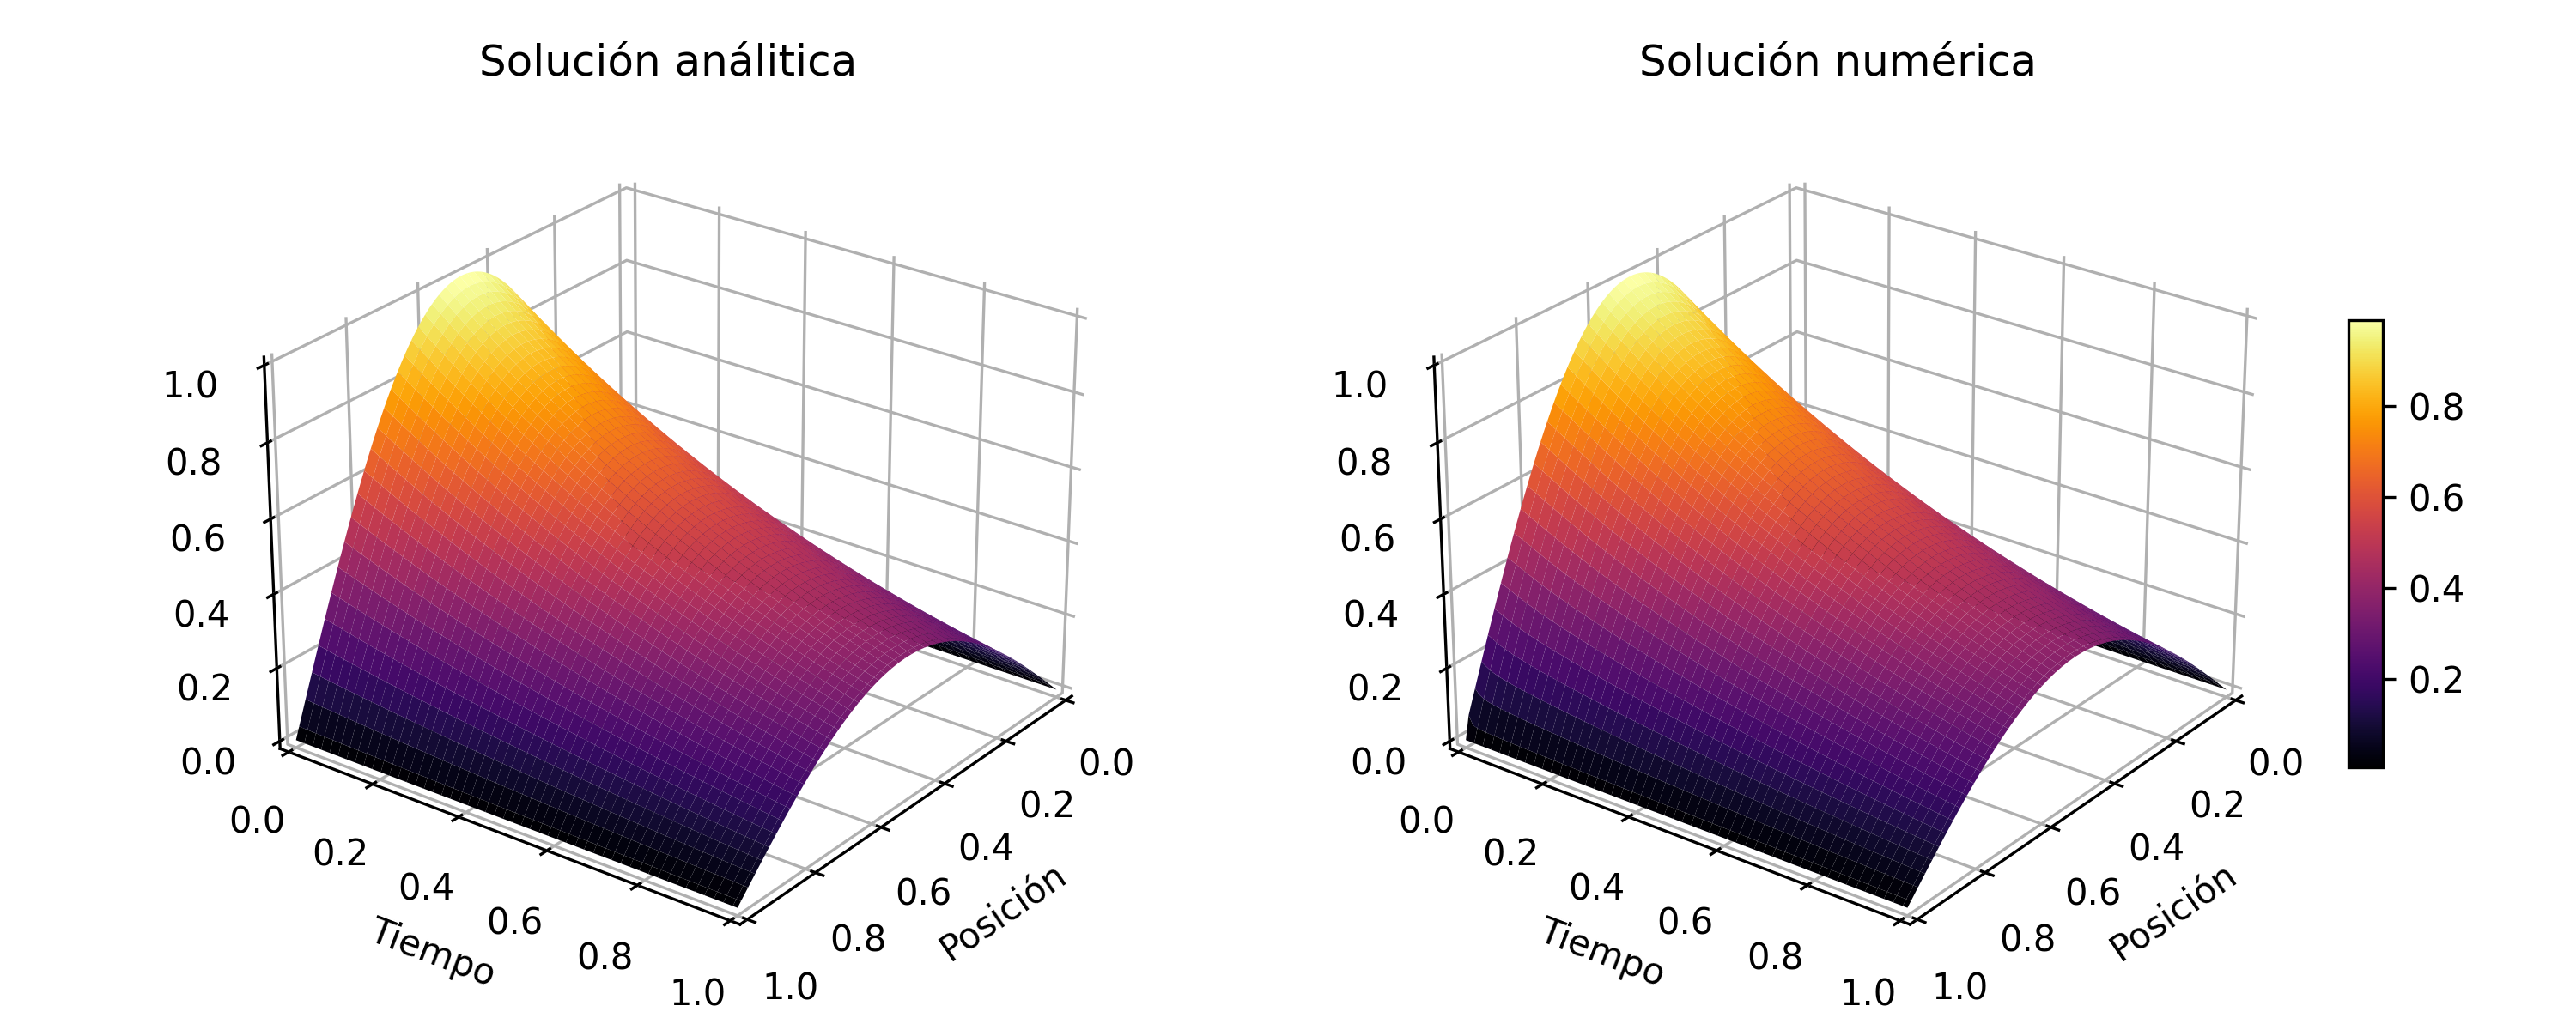
\includegraphics[width=17cm]{Graphics/surface_2.png}
	\caption{Solución análitica y numérica de la ecuación \ref{eq:heat_2} bajo las condiciones de frontera de la ecuación \ref{eq:bound_2}.}
	\label{fig:sol_2}
\end{figure}

\subsection{Dataset 3}

Se tiene la siguiente ecuación diferencial parcial:

\begin{equation}
	\frac{\partial u}{\partial t} = \frac{\partial^2 u}{\partial x^2}+10x(1-x)cos(10t)+2sin(10t)\qquad 0<x<1, \; t>0 \label{eq:heat_3}
\end{equation}

con las siguientes condiciones de frontera:
\begin{equation}
	\begin{cases}
		u(x,0) & = sin(\pi x) \qquad 0<x<1 \\
		u(0,t) & =u(1,t) = 0, \qquad t>0
	\end{cases} \label{eq:bound_3}
\end{equation}

La solución análitica de este conjuntos de ecuaciones es:

\begin{equation}
	u(x,t)= e^{-\pi^2 t}sin(\pi x)+x(1-x)sin(10t) \label{eq:sol_3}
\end{equation}

En la figura \ref{fig:sol_3} se muestra la solución análitica y numérica de la ecuación \ref{eq:bound_3} bajo las conficiones de frontera de la ecuación \ref{eq:bound_3}. La diferencia relativa entre los dos resultados es de 0.4409\%, dando así una gran similitud entre los dos resultados.

\begin{figure}[H]
	\centering
	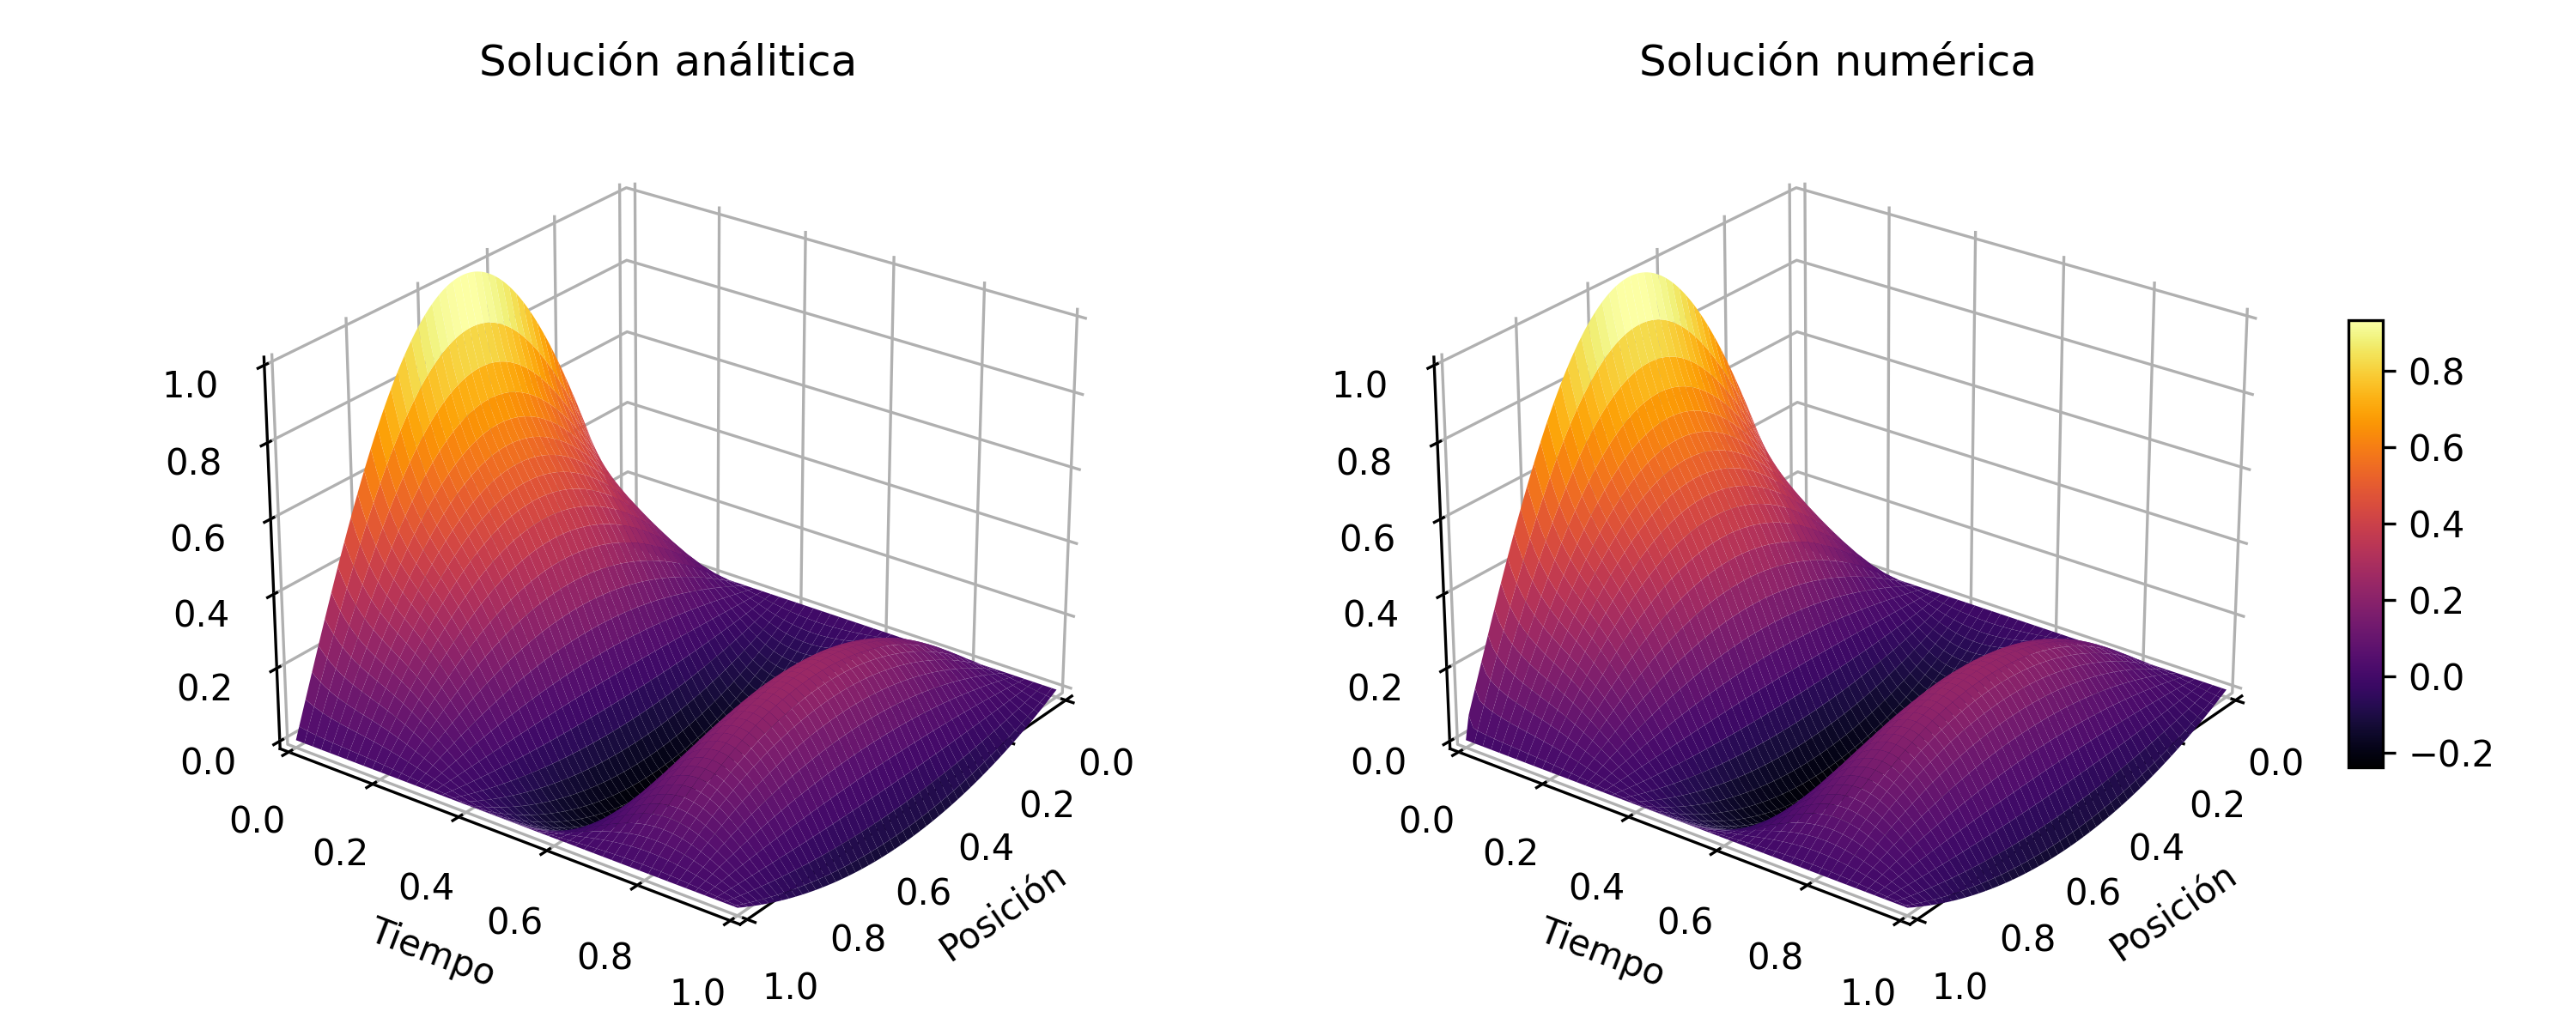
\includegraphics[width=17cm]{Graphics/surface_3.png}
	\caption{Solución análitica y numérica de la ecuación \ref{eq:heat_3} bajo las condiciones de frontera de la ecuación \ref{eq:bound_3}.}
	\label{fig:sol_3}
\end{figure}

\subsection{Dataset 4}

Se tiene la siguiente ecuación diferencial parcial:

\begin{equation}
	\frac{\partial u}{\partial t} = 4\frac{\partial^2 u}{\partial x^2}+e^tsin(x)\qquad 0<x<\pi, \; t>0 \label{eq:heat_4}
\end{equation}

con las siguientes condiciones de frontera:
\begin{equation}
	\begin{cases}
		u(x,0) & = sin(\pi x) \qquad 0<x<1 \\
		u(0,t) & =u(\pi,t) = 0, \qquad t>0
	\end{cases} \label{eq:bound_4}
\end{equation}

La solución análitica de este conjuntos de ecuaciones es:

\begin{equation}
	u(x,t)=\frac{1}{5}( e^t-e^{-4t})sin(x) \label{eq:sol_4}
\end{equation}


\begin{figure}[H]
	\centering
	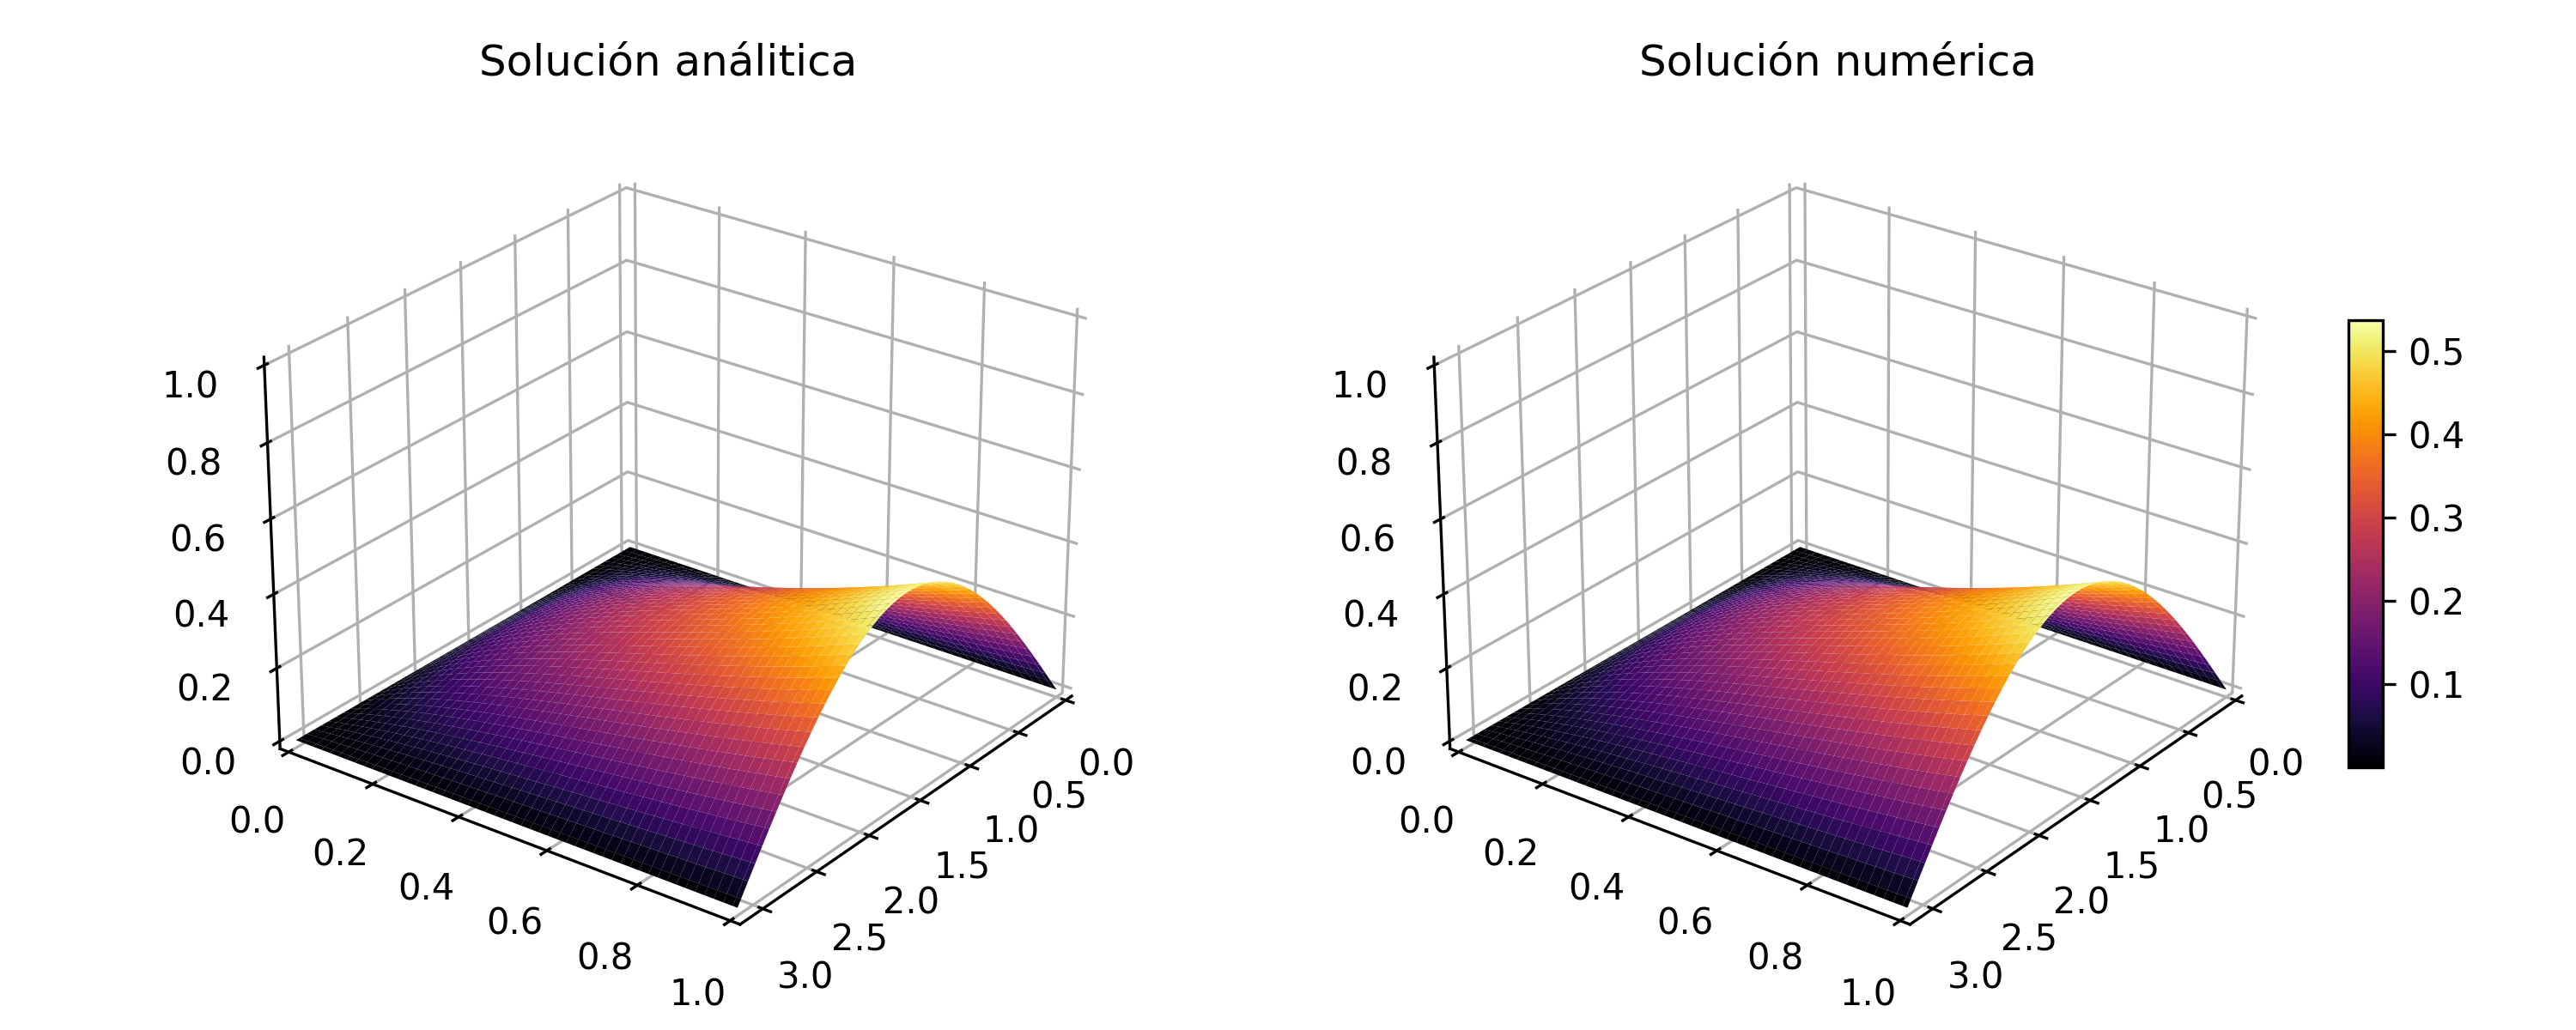
\includegraphics[width=17cm]{Graphics/surface_4.png}
	\caption{Solución análitica y numérica de la ecuación \ref{eq:heat_4} bajo las condiciones de frontera de la ecuación \ref{eq:bound_4}.}
	\label{fig:sol_4}
\end{figure}

En la figura \ref{fig:sol_4} se muestra la solución análitica y numérica de la ecuación \ref{eq:bound_4} bajo las conficiones de frontera de la ecuación \ref{eq:bound_4}. La diferencia relativa entre los dos resultados es de 0.0997\%, dando así una gran similitud entre los dos resultados.
